\documentclass{article}
\usepackage{tikz}
\usepackage{fontspec}
\setmainfont{IBM Plex Mono}

\begin{document}

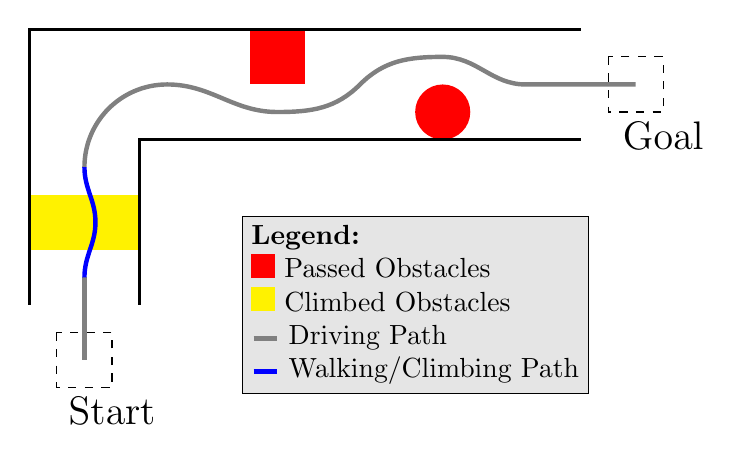
\begin{tikzpicture}[scale=0.7]

    % Obstacles
    \fill[red] (-6,-1) rectangle (-5,0);
    \fill[red] (-2.5,-1.5) circle (0.5);
    \fill[yellow] (-10,-4) rectangle (-8,-3);
    
    % Walls
    \draw[very thick] (0,0) -- (-10,0) -- (-10,-5);
    \draw[very thick] (0,-2) -- (-8,-2) -- (-8, -5);
    
    % Start
    \draw [black,dashed] (-9.5,-5.5) rectangle (-8.5,-6.5) node [black,below] {\Large Start};
    
    % Goal
    \draw [black,dashed] (0.5,-0.5) rectangle (1.5,-1.5) node [black,below] {\Large Goal};
    
    % Driving Path
    \draw [gray, ultra thick] (1,-1) % Draws a line
      to [out=180,in=0] (-1,-1) %Line
      to [out=180,in=0] (-2.5,-0.5) %Arc
      to [out=180,in=45] (-4,-1) %Arc
      to [out=225,in=0] (-5.5,-1.5) %Arc
      to [out=180,in=0] (-7.5,-1) %Arc
      to [out=180,in=90] (-9,-2.5) %Arc
      ;
    \draw[gray, ultra thick] (-9,-4.5) -- (-9,-6);
    
    % Walking Path
    \draw [blue,ultra thick] (-9,-2.5)
    to [out=270,in=90] (-8.8,-3.5)
    to [out=270,in=90] (-9,-4.5)
    ;

    % Legend
    \node[draw, fill=gray!20, minimum width=4cm, minimum height=2cm, align=left] (notationBox) at (-3,-5) {
    \textbf{Legend:} \\ 
    \tikz\fill[red] (0,0) rectangle (0.3cm,0.3cm); Passed Obstacles\\
    \tikz\fill[yellow] (0,0) rectangle (0.3cm,0.3cm); Climbed Obstacles\\
    \tikz[baseline=-0.5ex]\draw[gray, ultra thick] (0,0) -- (0.3,0); Driving Path\\
    \tikz[baseline=-0.5ex]\draw[blue, ultra thick] (0,0) -- (0.3,0); Walking/Climbing Path
    };
    
\end{tikzpicture}

\end{document}